\documentclass[a4paper,11pt]{article}

% Kodovani (cestiny) v dokumentu: utf-8
%\usepackage[cp1250]{inputenc}	% Omezena stredoevropska kodova stranka, pouze MSW.
\usepackage[utf8]{inputenc}	% Doporucujeme pouzivat UTF-8 (unicode).

\usepackage[margin=2cm]{geometry}
\newtoks\jmenopraktika \newtoks\jmeno \newtoks\datum
\newtoks\obor \newtoks\skupina \newtoks\rocnik \newtoks\semestr
\newtoks\cisloulohy \newtoks\jmenoulohy
\newtoks\tlak \newtoks\teplota \newtoks\vlhkost

\jmenopraktika={Fyzikální praktikum 1}
\jmeno={Lukáš Lejdar}
\datum={5. března 2024}
\obor={F}
\skupina={Út 16:00}

\cisloulohy={2}
\jmenoulohy={Měření odporu rezistoru}

\tlak={101{,}35}
\teplota={24,1}
\vlhkost={26,6}


%%%%%%%%%%% Uzitecne balicky:
\usepackage[czech]{babel}
\usepackage{graphicx}
\usepackage{amsmath}
\usepackage{xspace}
\usepackage{url}
\usepackage{indentfirst}
\usepackage{wrapfig}

%%%%%% Zamezeni parchantu:
\widowpenalty 10000 \clubpenalty 10000 \displaywidowpenalty 10000
%%%%%% Parametry pro moznost vsazeni vetsiho poctu obrazku na stranku
\setcounter{topnumber}{3}	  % max. pocet floatu nahore (specifikace t)
\setcounter{bottomnumber}{3}	  % max. pocet floatu dole (specifikace b)
\setcounter{totalnumber}{6}	  % max. pocet floatu na strance celkem
\renewcommand\topfraction{0.9}	  % max podil stranky pro floaty nahore
\renewcommand\bottomfraction{0.9} % max podil stranky pro floaty dole
\renewcommand\textfraction{0.1}	  % min podil stranky, ktery musi obsahovat text
\intextsep=8mm \textfloatsep=8mm  %\intextsep pro ulozeni [h] floatu a \textfloatsep pro [b] or [t]

% Tecky za cisly sekci:
\renewcommand{\thesection}{\arabic{section}.}
\renewcommand{\thesubsection}{\thesection\arabic{subsection}.}
% Jednopismenna mezera mezi cislem a nazvem kapitoly:
\makeatletter \def\@seccntformat#1{\csname the#1\endcsname\hspace{1ex}} \makeatother
%
\newcommand{\vsn}[4]{\ensuremath{#1 =} #2(#3)\,#4}
\newcommand{\vrn}[6]{\ensuremath{#1 =} (#2 $\pm$ #3)\,#4 ($p=$ #5\,\%, $\nu=$ #6)}


%%%%%%%%%%%%%%%%%%%%%%%%%%%%%%%%%%%%%%%%%%%%%%%%%%%%%%%%%%%%%%%%%%%%%%%%%%%%%%%
% Zacatek dokumentu
%%%%%%%%%%%%%%%%%%%%%%%%%%%%%%%%%%%%%%%%%%%%%%%%%%%%%%%%%%%%%%%%%%%%%%%%%%%%%%%

\begin{document}

\thispagestyle{empty}

{
\begin{center}
\sf 
{\Large Ústav fyziky a technologií plazmatu Přírodovědecké fakulty Masarykovy univerzity} \\
\bigskip
{\huge \bfseries FYZIKÁLNÍ PRAKTIKUM} \\
\bigskip
{\Large \the\jmenopraktika}
\end{center}

\bigskip

\sf
\noindent
\setlength{\arrayrulewidth}{1pt}
\begin{tabular*}{\textwidth}{@{\extracolsep{\fill}} l l}
\large {\bfseries Zpracoval:}  \the\jmeno & \large  {\bfseries Naměřeno:} \the\datum\\[2mm]
\large  {\bfseries Obor:} \the\obor  \hspace{40mm}  {\bfseries Skupina:} \the\skupina %
&\large {\bfseries Testováno:}\\
\\
\hline
\end{tabular*}
}

\bigskip

{
\sf
\noindent \begin{tabular}{p{4cm} p{0.6\textwidth}}
\Large  Úloha č. {\bfseries \the\cisloulohy:} \par
\smallskip
$T=\the\teplota$~$^\circ$C \par
$p=\the\tlak$~kPa \par
$\varphi=\the\vlhkost$~\%
&\Large \bfseries \the\jmenoulohy  \\[2mm]
\end{tabular}
}

\vskip1cm

\section{Úvod}
\begin{enumerate}
  \item Máme za úkol nepřímo změřit odpor dvour rezistorů pomocí ampermetru a voltmetru, použitím vztahu
    \begin{equation}
      \label{eq:1}
      R = \frac{U_R}{I_R},
    \end{equation}
  kde $U_R$ je napětí a $I_R$ proud, který odporem protéká.
  \item Druhou částí úlohy je změřit voltamperovou charakteristiku žárovky.
\end{enumerate}

\section{Postup měření} 

K měření napětí je zapotřebí voltmetr zapojený paralelně k odporu, zatímco měření ampermetrem vyžaduje seriové zapojení.
Máme tedy 2 možnosti navržení obvodu, tak abychom obě veličny měřili zároveň

\begin{figure}[htbp]
  \begin{minipage}[t]{0.45\textwidth}
    \centering
    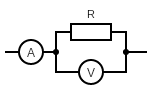
\includegraphics[width=5cm]{circuitA.png}
    \caption{Schéma zapojení metodou A}%
  \end{minipage}
  \hfil
  \begin{minipage}[t]{0.45\textwidth}
    \centering
    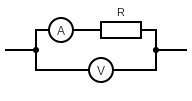
\includegraphics[width=5cm]{circuitB.png}
    \caption{Schéma zapojení metodou B}%
  \end{minipage}
\end{figure}

Ampermetr ale v zapojení A neměří proud přímo, měří proud i na Voltmeru $I_A = I_V + I_R$ . 
Obdobně u metody B, $U_V = U_A + U_R$ . Dosazením do vzorečků dostáváme, \\

\begin{align}
  \label{eq:2}
  \text{Metodou A} & & R &= \frac{U_R}{I_R} = \frac{U_V}{I_A - \frac{U_V}{R_V}} & & \\[5pt]
  \label{eq:3}
  \text{Metodou B} & & R &= \frac{U_V}{I_R} = \frac{U_V - R_AI_A}{I_A} = \frac{U_V}{I_A} - R_A & &
\end{align}

Kterou metodu zvolit? Naším cílem je provést měření co nejpřesněji, tedy získat odchylku $u(R)$ co nejmenší.
Lze ukázat, že metoda A bude výhodnější pro odpory, které jsou relativně mnohem menší než odpor Voltmetru, $R \ll R_V$, 
zatímco metoda B bude výhodnější pokud odpor Ampermetru, je mnohem menší, než měřený odpor $R_A \ll R$. 
V úloze měříme 2 různé odpory oběma způsoby a nakonec porovnáme výsledky. \\

K měření jsme použili tyto přístroje
\begin{itemize}
    \item stolní Multimetr U3402A - pro měření proudu ($R_A=\frac{150}{12}$ $\Omega$)
    \item ruční multimer ESCORT - pro měření napětí ($R_V=10$ $M\Omega$)
\end{itemize}

\section{Výsledky měření}

\subsection{Měření odporů}

Naměřené hodnoty oběma metodami jsou spolu s aritmetickým průměrem a nejistotou uvedeny v~tabulce \ref{tb:mer}.

\begin{table}[ht]
  \centering
  \begin{tabular}{ c | c | c | c | c }
     & \multicolumn{2}{c |}{Metoda A} & \multicolumn{2}{c}{Metoda B} \\ \hline\hline
    Odpor & $R_1$ & $R_2$ & $R_1$ & $R_2$ \\ \hline
    $I_A$ [mA] & 30.36 $\pm$ 2 & 0.017 $\pm$ 2 & 54.74 $\pm$ 3 & 0.016 $\pm$ 2 \\
    $U_V$ [V] & 3.000 $\pm$ 5 & 16.00 $\pm$ 2 & 6.000 $\pm$ 8 & 16.16 $\pm$ 2 \\ \hline\hline
    Vztah (1) & 98.9 $\pm$ 0.2 [$\Omega$] & 0.9 $\pm$ 0.1 [M$\Omega$] & 109.6 $\pm$ 0.2 [$\Omega$] & 1.0 $\pm$ 0.1 [M$\Omega$] \\
    Vztah (2) a 3 & 98.8 $\pm$ 0.2 [$\Omega$] & 1.0 $\pm$ 0.1 [M$\Omega$] & 97.1 $\pm$ 0.2 [$\Omega$] & 1.0 $\pm$ 0.1 [M$\Omega$] \\

  \end{tabular}
  \caption{Naměřené hodnoty}
  \label{tb:mer}
\end{table}

\subsection{Měření voltamperové charakteristiky žárovky}

\begin{figure}[htpb]
  \centering
  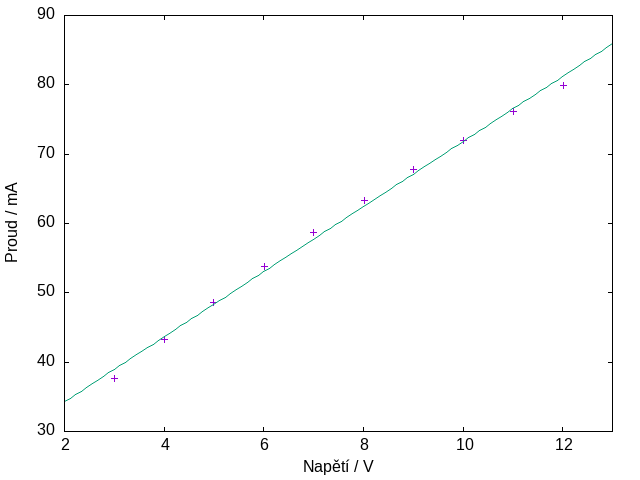
\includegraphics[width=0.7\linewidth]{zarovka-graf.png}
  \caption{graf voltamperové charakteristiky žárovky}
\end{figure}


\section{Závěr} 

Z tabulky 1 je vidět, že použití metody A je pro menší odpory opravud vhodnější, zatímco metoda B je lepší pro ty větší.
Bez velké ztráty přsnosti bychom mohli výpočet provést přímo z Ohmova zákona.
Voltamperova charakteristika žárovky nasvědšuje malou nelinearitu, ale myslím že efekt by 
byl zřetelnější pro větší rozsah měření napětí.



\begin{thebibliography}{0}
\bibitem{navody} Bochníček a kol. \textit{Fyzikální praktikum 1, návody k ulohám.} Brno 2024.\\ Dostupné z~\url{https://monoceros.physics.muni.cz/kof/vyuka/fp1_skripta.pdf}.   
\bibitem{tabulky} Hustota pevných látek. Dostupné z~\url{http://www.converter.cz/tabulky/hustota-pevne.htmf}.   
\end{thebibliography}

\end{document}
